Most of the braille display products available in the market right now, such as those sold by HumanWare and RNIB, are based on piezoelectric bimorph benders or relay-lever mechanisms.  

The biomorph benders mechanism, shown in figure \ref{fig:piezo-bender} produces vibrations that move the pin up and down when placed in an electric field.
In relay-lever mechanisms, shown in figure \ref{fig:piezo-relay}, when voltage is supplied, the relay pushes the pin up. When the power is off, the weight of the lever mechanism moves the pin downwards to its original position. \cite{hernandez_characterization_2009}.

\begin{figure} \centering
    \begin{subfigure}[b]{0.4\textwidth}\centering
        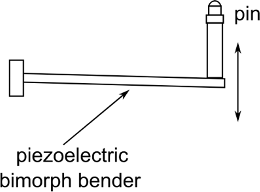
\includegraphics[height=3cm]{figures/piezo-bender-a.png}
        \caption{}
        \label{fig:piezo-bender}
    \end{subfigure}
    \begin{subfigure}[b]{0.4\textwidth}\centering
        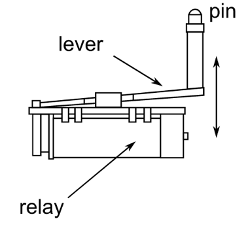
\includegraphics[height=3.5cm]{figures/piezo-bender-b.png}
        \caption{}
        \label{fig:piezo-relay}
    \end{subfigure}
\caption{Examples of existing Braille mechanisms: (a) piezoelectric bimorph bender and (b) relay-lever system \cite{hernandez_characterization_2009}.}
\label{fig:piezo-bender-schema}
\end{figure}

\todo[inline]{This moves from describing mechanism to condemning it. Requires information on what makes it burdensome, what is the cost and/or more concrete disadvantage why it's excluded.}
The main drawback of these two popular mechanisms is that the functional modules are burdensome and must be placed directly under pins. Therefore, it is hard to make portable devices with these mechanisms and the expensive cost of producing one line of cells also limits the number of lines available. 

Another recently developed mechanism is piezoelectric ultrasonic motor \cite{hernandez_characterization_2009}.
The ultrasonic linear motor consists of a shaft, a mobile element or slider, and a piezoelectric ceramic disk as shown in figure \ref{fig:piezo-miniature}.
The key advantage of this design is the ultra-light weight of this miniature motor.
However, the need for several layers, as shown in figure \ref{fig:piezo-full-design}, does not befit the density required by a 2D tactile display.

\begin{figure}[h] \centering
    \begin{subfigure}[b]{0.45\textwidth}\centering
        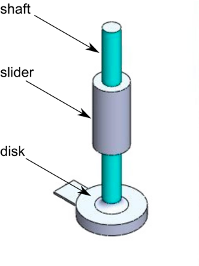
\includegraphics[height=5cm]{figures/piezo-miniature-a.png}
        \caption{}
        \label{fig:piezo-miniature-a}
    \end{subfigure}
    \begin{subfigure}[b]{0.45\textwidth}\centering
        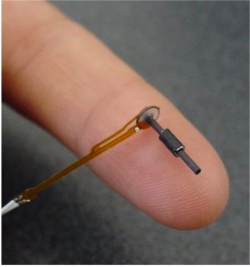
\includegraphics[height=5cm]{figures/piezo-miniature-b.png}
        \caption{}
        \label{fig:piezo-miniature-b}
    \end{subfigure}
\caption[Miniature piezoelectric linear motor]{Miniature piezoelectric linear motor: (a) conceptual design and (b) prototype.}
\label{fig:piezo-miniature}
\end{figure}

\begin{figure}\centering
    \begin{subfigure}[b]{0.45\textwidth}\centering
        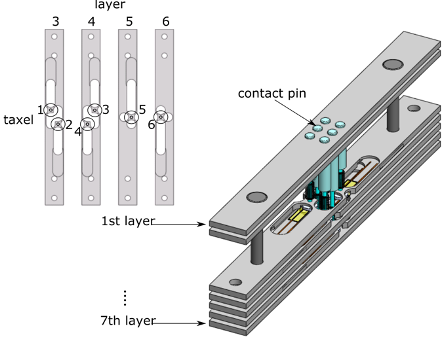
\includegraphics[height=5cm]{figures/piezo-full-design-a.png}
        \caption{}
    \end{subfigure}
    \begin{subfigure}[b]{0.45\textwidth}\centering
        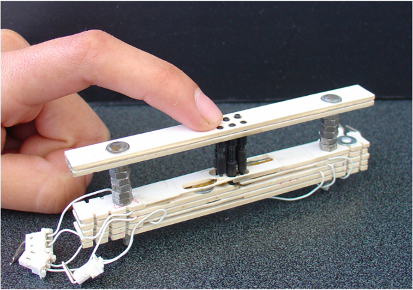
\includegraphics[height=4cm]{figures/piezo-full-design-b.png}
        \caption{}
    \end{subfigure}
\caption{}
\label{fig:piezo-full-design}
\end{figure}